% Author Name: José Areia 
% Author Contact: jose.apareia@gmail.com
% Version: 1.0.3 - 18/04/2025
% Public Repository: https://github.com/joseareia/nob-article

% Packages & Document Configurations
\documentclass[onecolumn]{NobArticle}
\usepackage{float}
\usepackage{booktabs}
\usepackage{pgfplots}
\usepackage{etoolbox} % for \newcounter and \stepcounter

\usepgfplotslibrary{external}
\tikzexternalize

\runninghead{Shortened Running Article Title}
\footertext{\textit{Journal X} (2023) 12:684}

% Title
\title{BLADE: Bug Localization Assisted Debugging Engine}

% Authors
\author{
    Pooria Roy\textsuperscript{1,3}, 
    Mariam El Mezouar\textsuperscript{2,3}
}

% Affiliations
\date{
    \textsuperscript{\textbf{1}}School of Computing, Queen's University, Kingston, Canada \\
    \textsuperscript{\textbf{2}}Faculty of Arts and Science, Queen's University, Kingston, Canada \\
    \textsuperscript{\textbf{2}}Department of Computer Science, Royal Military College of Canada, Kingston, Canada
}

% % Abstract
% \renewcommand{\maketitlehookd}{%
% \begin{abstract}
%     \noindent Lorem ipsum dolor sit amet, consectetur adipiscing elit. Praesent porttitor arcu luctus, imperdiet urna iaculis, mattis eros. Pellentesque iaculis odio vel nisl ullamcorper, nec faucibus ipsum molestie. Sed dictum nisl non aliquet porttitor. Etiam vulputate arcu dignissim, finibus sem et, viverra nisl. Aenean luctus congue massa, ut laoreet metus ornare in. Nunc fermentum nisi imperdiet lectus tincidunt vestibulum at ac elit. Nulla mattis nisl eu malesuada suscipit. Aliquam arcu turpis, ultrices sed luctus ac, vehicula id metus. Morbi eu feugiat velit, et tempus augue. Proin ac mattis tortor. Donec tincidunt, ante rhoncus luctus semper, arcu lorem lobortis justo, nec convallis ante quam quis lectus. Aenean tincidunt sodales massa, et hendrerit tellus mattis ac. Sed non pretium nibh. Donec cursus maximus luctus. Vivamus lobortis eros et massa porta porttitor.
% \end{abstract}
% }

\begin{document}

\small
\maketitle

% Introduction
\section{Introduction}
Recent advances in Large Language Models (LLMs) have introduced new possibilities for Automated Program Repair (APR). By understanding code context and iteratively testing their own fixes, LLMs can reduce the need for human intervention. This becomes more prominent in smaller projects, where the limited number of files and lines of code allows the entire context to fit within the model's input window.\\
However, this advantage diminishes as the size and complexity of a project grow. While larger codebases may technically fit within the context window, effective bug localization requires more than surface-level pattern recognition. It demands a deeper, semantic understanding of program behavior and structure something current LLMs are still not fully equipped to handle.\\
To address these limitations, we propose a pipeline that localizes bugs without relying on LLMs. By analyzing the codebase in tandem with the error trace, our method can more precisely identify the source of a bug. It comes within 3\% of the performance of Blaze (the current state-of-the-art). 
In our evaluation, this approach outperforms strategies that simply feed the full codebase to an LLM, offering a more scalable solution to the problem.

\begin{figure}[H]
\centering
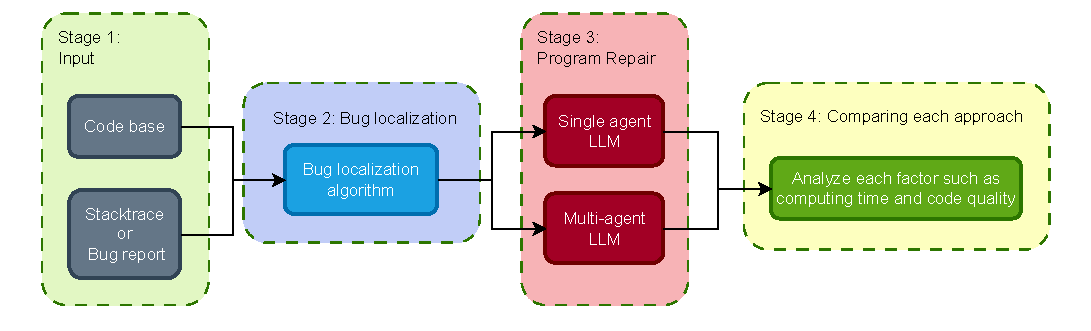
\includegraphics[width=1\columnwidth]{Figures/OverallView.pdf}
\caption{APR Pipeline}
\label{fig:apr_pipeline}
\end{figure}

\section{Related Work}
Recent approaches to bug localization increasingly use code embeddings to represent both source files and failure contexts, such as stack traces or bug reports in a shared semantic space for similarity-based retrieval.\\
Early models like the DNN+IR hybrid from \citet{7961519} combined keyword-based search with a deep neural network, achieving around 85\% Top-20 accuracy. xLoc \citep{yang2024xloc} leverages a multilingual Transformer to classify buggy functions and localize errors, reaching 87.54\% Top-1 accuracy.\\
BLAZE \citep{blaze2024} uses the CodeSage model \citet{zhang2024coderepresentationlearningscale} to embed entire codebases and bug reports. It applies dynamic chunking and combines semantic and lexical retrieval to support cross-project localization, achieving 60-70\% Top-20 accuracy.\\
BugLLM \citep{subramanian2024bugllm} takes a zero-shot approach, generating natural language queries with an LLM and retrieving relevant code chunks via embeddings. It reports 44.7-61.1\% Top-5 accuracy, with explanation rated highly for clarity and correctness.
\section{Inputs}

\begin{figure}[H]
\centering
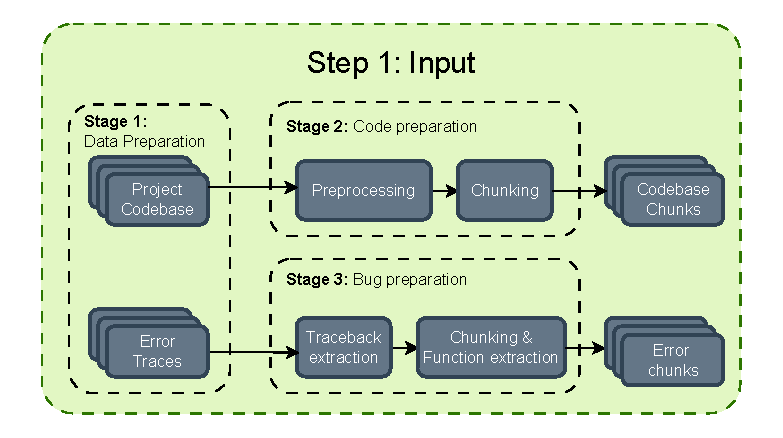
\includegraphics[width=1\columnwidth]{Figures/Step1_input.drawio.pdf}
\caption{Input processing}
\label{fig:step1_input}
\end{figure}


\subsection{Data Preparation}
Selecting an appropriate dataset is key to evaluating the pipeline. We use an enhanced version of the BugsInPy dataset \citep{aguilar2023reproducing}, which improves reproducibility by providing validated Docker environments for each bug. Projects were selected based on criteria that ensures diversity and sufficient number of bug cases. An overview of the selected projects is provided in Table~\ref{tab:bugsinpy_projects}

\begin{table}[H]
\centering
\begin{tabularx}{\textwidth}{lcccccccc}
\toprule
\textbf{Projects} & \textbf{Bugs} & \textbf{Avg. Trace LoC} & \textbf{Min. Trace LoC} & \textbf{Max. Trace LoC} & \textbf{File count} & \textbf{Avg. LoC} & \textbf{Min. LoC} & \textbf{Max. LoC} \\
\midrule
matplotlib & 23 & 91.2 & 49 & 232 & 762 & 244.3 & 1 & 8054 \\
pandas & 124 & 261.2 & 30 & 4375 & 297 & 602.8 & 1 & 11407 \\
youtube-dl & 31 & 26.3 & 2 & 56 & 809 & 159.7 & 4 & 3888 \\
luigi & 30 & 84.2 & 27 & 319 & 119 & 261.3 & 17 & 1647 \\
black & 19 & 138.5 & 18 & 591 & 23 & 4134.5 & 2 & 41441 \\
scrapy & 37 & 33.7 & 18 & 133 & 177 & 100.5 & 1 & 531 \\
thefuck & 30 & 84.8 & 27 & 363 & 198 & 33.6 & 1 & 338 \\
keras & 34 & 375.9 & 79 & 3476 & 135 & 362.8 & 1 & 4494 \\
ansible & 135 & 74.8 & 12 & 246 & 582 & 236.9 & 1 & 3446 \\
\bottomrule
\end{tabularx}
\caption{Projects chosen from BugsInPy dataset}
\label{tab:bugsinpy_projects}
\end{table}


\subsection{Code preparation}
Before embedding, we preprocess each project by cloning its repository and filtering out non-source files (e.g., tests, configuration scripts, and data). To handle long source files and improve semantic focus, we apply an AST-based chunking strategy. Using Python's built-in Abstract Syntax Tree (AST) module, we split each file into logical units corresponding to top-level classes and functions. This reduces noise from unrelated code and ensures that the resulting chunks are semantically meaningful.
\subsection{Bug preparation}
As part of bug preprocessing, we extract the relevant segments of each tracebacks by removing non-informative frames, such as logging calls and third-party utility layers. This refinement improves the overall success rate by 3\%. To ensure clear evaluation targets, we include only bugs where exactly one file is modified, based on the available ground truth.

\section{Bug Localization}
\begin{figure}[H]
\centering
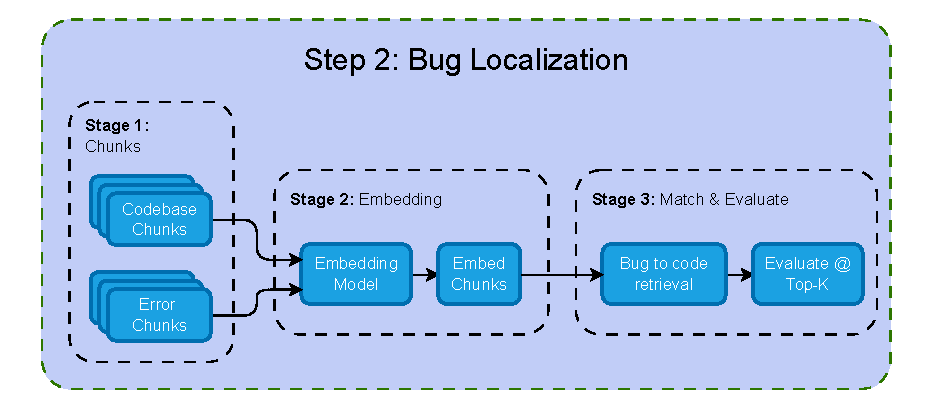
\includegraphics[width=1\columnwidth]{Figures/Step2_bug_localization.drawio.pdf}
\caption{Bug localization pipeline}
\label{fig:step2_bug_localization}
\end{figure}

\subsection{Model Selection and Performance}
Empirically, we find that smaller models trained specifically on code embeddings outperform both general-purpose language models and larger code models in our localization task. Table~\ref{tab:model_performance_at_k} summarizes the top-$k$ accuracy across several embedding models. We adopt the \texttt{blaze} model due to its strong performance and efficient resource usage; It supports batch sizes up to 128 on an 8GB GPU, compared to over 15GB required by larger models such as \texttt{jinaai/jina-embedding-v2-base-code} at batch size 2. Earlier experiments with \texttt{MiniLM-L12-v2} served as a baseline, yielding 60\% Top-5 accuracy.

\subsection{Retrieval Method}
For retrieval, we compute cosine similarity between the embedded bug trace and each code chunk, returning the top-$k$ most similar candidates. As shown in Figure~\ref{fig:blaze@k_graph}, performance improves significantly between $k=1$ and $k=10$.

\subsection{Dataset Characteristics}
We also observe that localization accuracy declines in projects with larger file counts. Table~\ref{tab:bugsinpy_projects} highlights that \texttt{pandas}, \texttt{matplotlib}, \texttt{ansible}, and \texttt{youtube-dl} have substantially larger codebases, and three of the four have reduced performance compared to other projects. This suggests that increasing the search space negatively impacts retrieval precision, even when using semantically rich embeddings.
\subsection{Evaluation Bias}
Table~\ref{fig:blaze@k_graph_file} presents top-$k$ accuracy based on the file name, while Table\ref{fig:blaze@k_graph_function} reports performance based on the function name.

\begin{figure}[H]
\centering
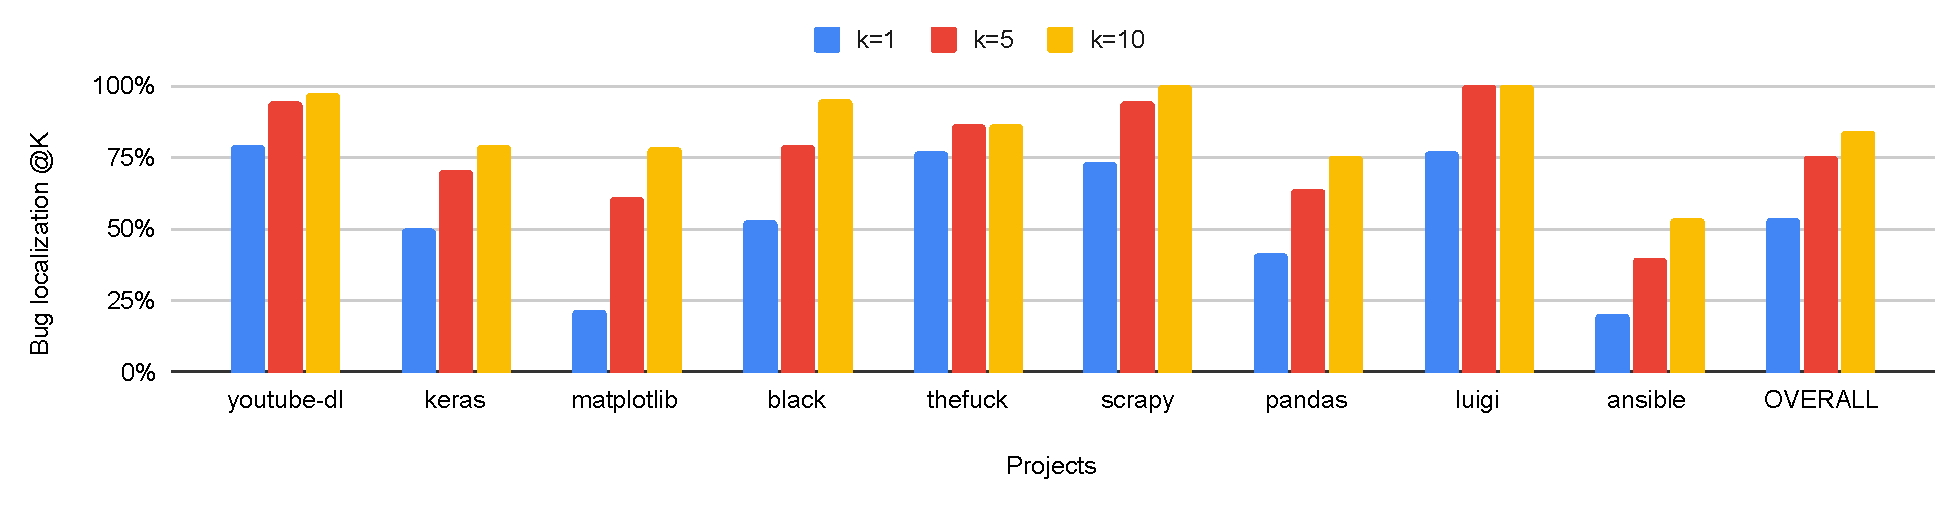
\includegraphics[width=1\columnwidth]{Figures/blaze@k_file.pdf}
\caption{File level bug localization accuracy @k for "blaze" a fine-tuned version of "codesage/codesage\_small\_v2"}
\label{fig:blaze@k_graph_file}
\end{figure}

\begin{figure}[H]
\centering
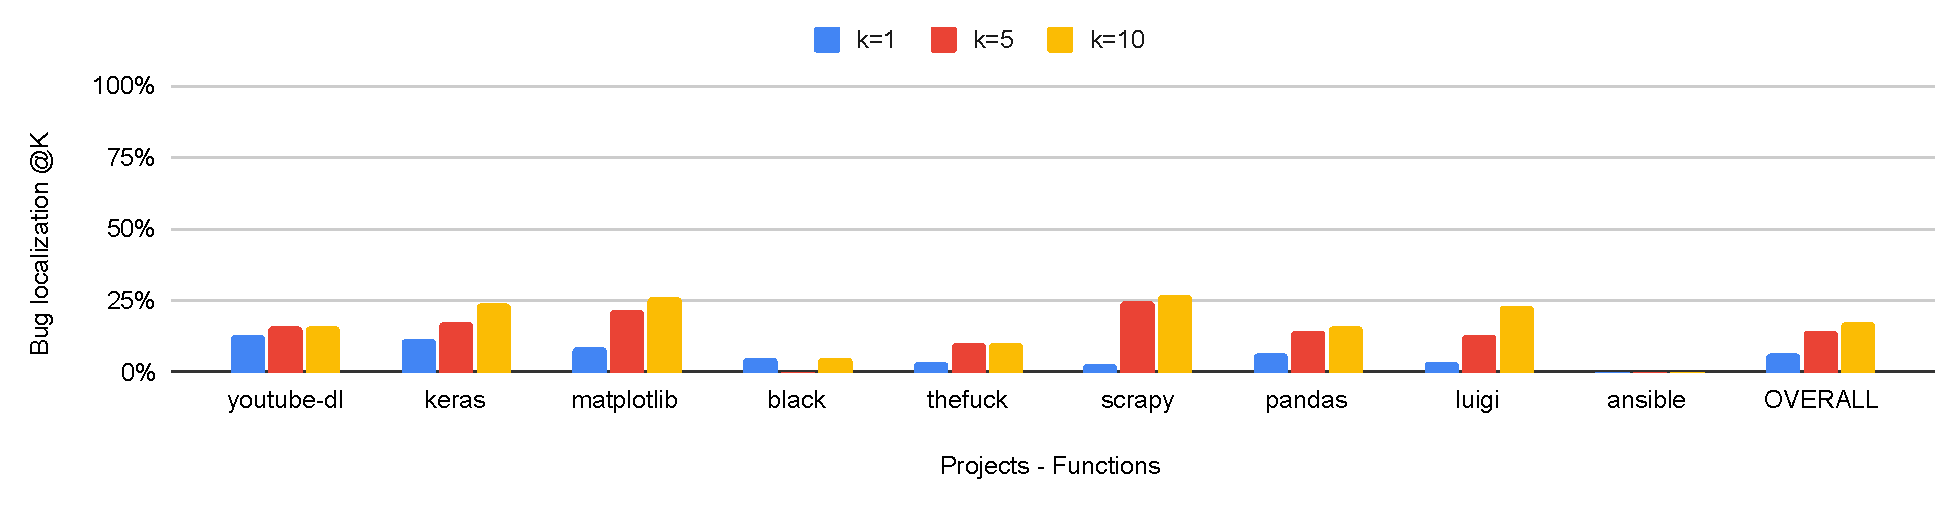
\includegraphics[width=1\columnwidth]{Figures/blaze@k_function.pdf}
\caption{Function level bug localization accuracy @k for "blaze" a fine-tuned version of "codesage/codesage\_small\_v2"}
\label{fig:blaze@k_graph_function}
\end{figure}

\begin{table}[H]
\centering
\begin{tabularx}{\textwidth}{lccccc}
\toprule
\textbf{Model} & \textbf{Top-1} & \textbf{Top-5} & \textbf{Top-10} & \textbf{MAP@60} & \textbf{MRR@60} \\
\midrule
BLAZE & 53.76\% & 75.43\% & 84.10\% & 40.81\% & 63.91\% \\
all-MiniLM-L12-v2 & 39.94\% & 63.85\% & 72.89\% & 32.15\% & 51.11\% \\
\bottomrule
\end{tabularx}
\caption{Overall success rate @k for different models at the file level}
\label{tab:model_performance_at_k}
\end{table}


\begin{table}[H]
\centering
\begin{tabularx}{\textwidth}{lccccc}
\toprule
\textbf{Model} & \textbf{Top-1} & \textbf{Top-5} & \textbf{Top-10} & \textbf{MAP@60} & \textbf{MRR@60} \\
\midrule
BLAZE & ?\% & ?\% & ?\% & ?\% & ?\% \\
\bottomrule
\end{tabularx}
\caption{Overall success rate @k for different models at the function level}
\label{tab:model_performance_at_k}
\end{table}

\section{APR}

\begin{figure}[H]
\centering
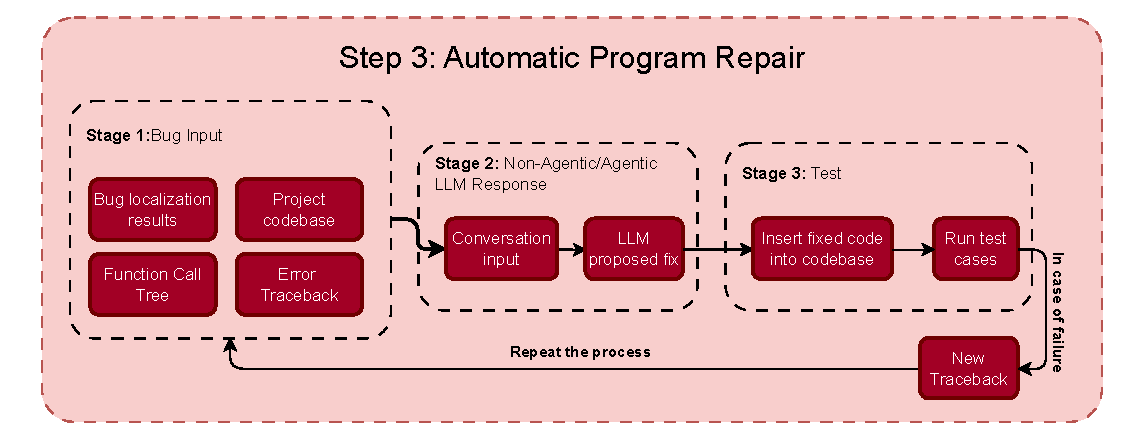
\includegraphics[width=1\columnwidth]{Figures/Step3_APR.drawio.pdf}
\caption{APR pipeline}
\label{fig:step2_bug_localization}
\end{figure}

LLMs are sensitive to the size and relevance of the input context. In practice, we found that providing entire source files—especially in legacy codebases where individual files may exceed 2,000 lines, substantially degrades the quality of repair suggestions. This is due to the dilution of relevant signal within overly broad inputs, often resulting in incoherent or incorrect fixes.

To address this limitation, we developed a targeted context-construction strategy that leverages both the error traceback and static code structure.

\subsection{Function Extraction from Error Traceback (Functional Call Tree)}

When a test case fails, we begin by analyzing the raw error traceback to identify all function calls that led to the failure. These functions are assumed to be highly relevant to the bug location. For each function, we retrieve the corresponding source code and extract any directly nested function calls within it (i.e., a call depth of 1). This process builds a partial call graph centered around the failing path.

\subsection{Reducing Context with Bug Localization (Not implemented yet)}
To further refine the set of candidate functions, we incorporate insights from the bug localization module. Functions that are deemed irrelevant based on localization confidence scores are discarded, ensuring that only high-signal code snippets are retained. The resulting context—comprising the error traceback and filtered function bodies is then provided to the LLM.

\subsection{Iterative Repair and Retesting}
The LLM generates a proposed fix based on the curated input. This fix is inserted directly into the codebase at the appropriate location. The modified code is then recompiled and retested. If the test fails again, the process is repeated using the new error traceback, allowing for up to three iterations. If no successful fix is found after three attempts, the process is terminated.

\subsection{Results}

\begin{table}[H]
\centering
\begin{tabularx}{\textwidth}{lccc}
\toprule
\textbf{Project} & \textbf{First Pass} & \textbf{Second Pass} & \textbf{Third Pass} \\
\midrule
youtube-dl & 48.64\% & 62.16\% & 72.22\% \\
\bottomrule
\end{tabularx}
\caption{Bug repair accuracy across multiple passes for the  projects}
\label{tab:apr_projects}
\end{table}

% \input{Sections/05-Discussion}
% \input{Sections/06-Conclusion}

\section{Reproducibility}
All code, scripts, and instructions required to reproduce our experiments are available in the BLADE repository\footnote{\url{https://github.com/regularpooria/BLADE}}. 
Data preparation and analysis scripts are included, along with detailed usage examples and Colab notebooks. 

\section*{Acknowledgments}
This research was conducted at the Royal Military College of Canada (RMC), Kingston, under the supervision of Professor Dr. El Mezouar. It was supported by the Natural Sciences and Engineering Research Council of Canada (NSERC).



\printbibliography

\end{document}
